\documentclass{article}

\usepackage{amsmath, amssymb}
\usepackage{array}
\usepackage[a3paper, margin=1in]{geometry}
%% landscape
\usepackage{tikz}
\usetikzlibrary{arrows}
\tikzset{
every picture/.style={very thick}
}

%%font
\usepackage{euler}
\usepackage[OT1]{eulervm}
\renewcommand{\rmdefault}{pplx}

\newcommand{\Var}{\operatorname{Var}}

\tikzset{
  byte/.pic={
    \draw (-2,-0.5) rectangle (2,0.5);
    \foreach \x in {-1.5,-1,...,1.5} {
      \draw (\x,-0.5) -- (\x,0.5);
    }
  }, 
  bytebox/.pic={
    \draw (-2,-0.5) rectangle (2,0.5);
  }
}

\begin{document}
%% absolute positioning
%% \begin{tikzpicture}[remember picture, overlay]
%%   \draw ([xshift=\x]current page.south) -- ([xshift=\x]current page.north);
%% \end{tikzpicture}    

\pagenumbering{gobble}

\begin{center}
  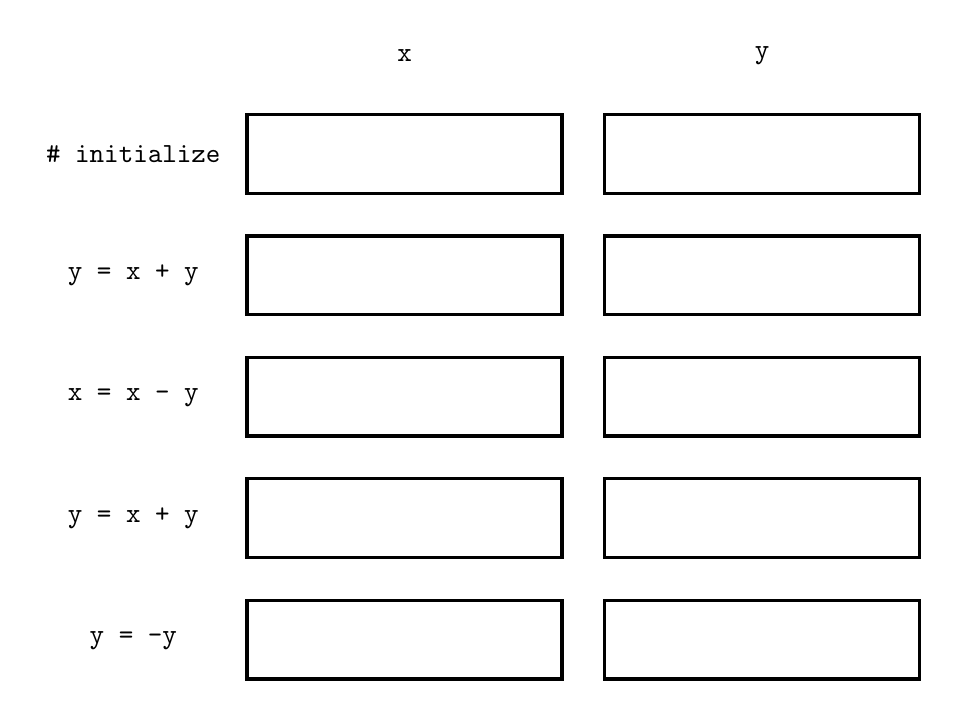
\begin{tikzpicture}
    \node[matrix, column sep=0.5cm, row sep=0.5cm] at (0,0) {
      &[-0.3cm] \node at (0,0) {\verb|x|}; & \node at (0,0) {\verb|y|}; \\
      \node at (0,0) {\verb|# initialize|}; & \pic at (0,0) {bytebox}; & \pic at (0,0) {bytebox}; \\
      \node at (0,0) {\verb|y = x + y|}; & \pic at (0,0) {bytebox}; & \pic at (0,0) {bytebox}; \\
      \node at (0,0) {\verb|x = x - y|}; & \pic at (0,0) {bytebox}; & \pic at (0,0) {bytebox}; \\
      \node at (0,0) {\verb|y = x + y|}; & \pic at (0,0) {bytebox}; & \pic at (0,0) {bytebox}; \\
      \node at (0,0) {\verb|y = -y|}; & \pic at (0,0) {bytebox}; & \pic at (0,0) {bytebox}; \\
    };
  \end{tikzpicture}
  \hfill
  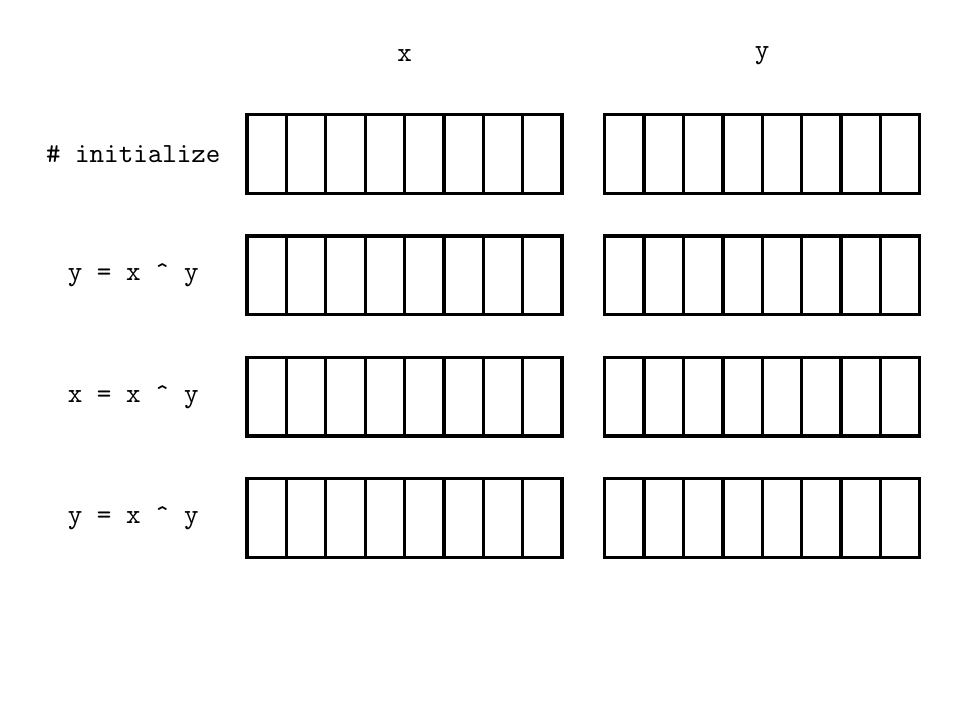
\begin{tikzpicture}
    \node[matrix, column sep=0.5cm, row sep=0.5cm] at (0,0) {
      &[-0.3cm] \node at (0,0) {\verb|x|}; & \node at (0,0) {\verb|y|}; \\
      \node at (0,0) {\verb|# initialize|}; & \pic at (0,0) {byte}; & \pic at (0,0) {byte}; \\
      \node at (0,0) {\verb|y = x ^ y|}; & \pic at (0,0) {byte}; & \pic at (0,0) {byte}; \\
      \node at (0,0) {\verb|x = x ^ y|}; & \pic at (0,0) {byte}; & \pic at (0,0) {byte}; \\
      \node at (0,0) {\verb|y = x ^ y|}; & \pic at (0,0) {byte}; & \pic at (0,0) {byte}; \\
      \node[opacity=0] at (0,0) {\verb|y = y|}; & \pic[opacity=0] at (0,0) {byte}; & \pic[opacity=0] at (0,0) {byte}; \\
    };
  \end{tikzpicture}  
\end{center}

\vspace{2cm}

\begin{description}
\item[Rule 1] $\rho_i \leftrightarrow \rho_j$ (not allowed)
\item[Rule 2] $\rho_i = k\rho_i$ for some $k\neq 0$
\item[Rule 3] $\rho_i = \rho_i + k\rho_j$
\end{description}

\begin{center}
  \begin{tikzpicture}
    \draw[opacity=0](0,-2) -- (0,2);
    \node at (0,0) {$\begin{bmatrix} 1 & 0 \\ 0 & 1 \end{bmatrix}$};
  \end{tikzpicture}
  \hfil
  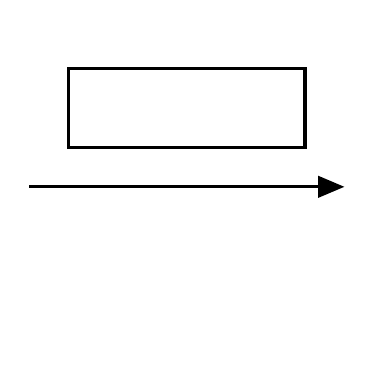
\begin{tikzpicture}
    \draw[opacity=0](0,-2) -- (0,2);
    \draw[-triangle 45] (-2,0) -- (2,0);
    \draw (-1.5,0.5) rectangle (1.5,1.5);
    \node[rectangle, opacity=0] at (0,1) {$\rho_2 = \rho_1 + \rho_2$};
  \end{tikzpicture}
  \hfil  
  \begin{tikzpicture}
    \draw[opacity=0](0,-2) -- (0,2);
    \node[opacity=0] at (0,0) {$\begin{bmatrix} 1 & 0 \\ 1 & 1 \end{bmatrix}$};
  \end{tikzpicture}
  \hfil
  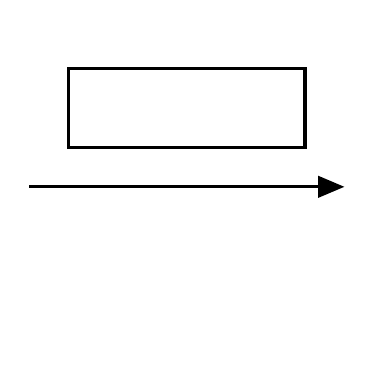
\begin{tikzpicture}
    \draw[opacity=0](0,-2) -- (0,2);
    \draw[-triangle 45] (-2,0) -- (2,0);
    \draw (-1.5,0.5) rectangle (1.5,1.5);
    \node[rectangle, opacity=0] at (0,1) {$\rho_1 = \rho_1 - \rho_2$};
  \end{tikzpicture}
  \hfil  
  \begin{tikzpicture}
    \draw[opacity=0](0,-2) -- (0,2);
    \node[opacity=0] at (0,0) {$\begin{bmatrix} 0 & -1 \\ 1 & 1 \end{bmatrix}$};
  \end{tikzpicture}
  \hfil
  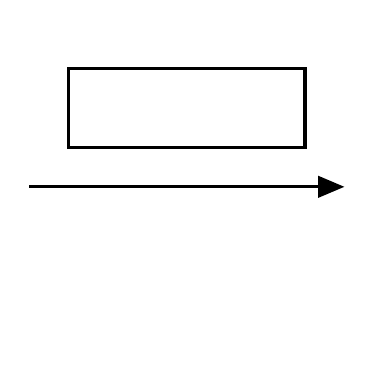
\begin{tikzpicture}
    \draw[opacity=0](0,-2) -- (0,2);
    \draw[-triangle 45] (-2,0) -- (2,0);
    \draw (-1.5,0.5) rectangle (1.5,1.5);
    \node[rectangle, opacity=0] at (0,1) {$\rho_2 = \rho_1 + \rho_2$};
  \end{tikzpicture}
  \hfil  
  \begin{tikzpicture}
    \draw[opacity=0](0,-2) -- (0,2);
    \node[opacity=0] at (0,0) {$\begin{bmatrix} 0 & -1 \\ 1 & 0 \end{bmatrix}$};
  \end{tikzpicture}
  \hfil
  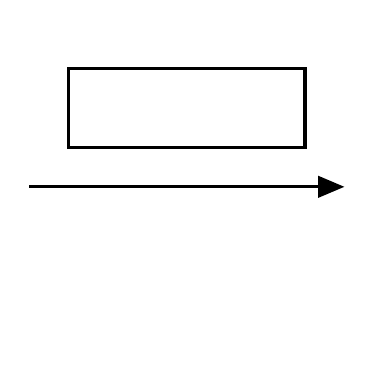
\begin{tikzpicture}
    \draw[opacity=0](0,-2) -- (0,2);
    \draw[-triangle 45] (-2,0) -- (2,0);
    \draw (-1.5,0.5) rectangle (1.5,1.5);
    \node[rectangle, opacity=0] at (0,1) {$\rho_1 = -\rho_1$};
  \end{tikzpicture}
  \hfil  
  \begin{tikzpicture}
    \draw[opacity=0](0,-2) -- (0,2);
    \node at (0,0) {$\begin{bmatrix} 0 & 1 \\ 1 & 0 \end{bmatrix}$};
  \end{tikzpicture}  
\end{center}

\vspace{2cm}

\begin{center}
  \begin{tabular}{c|cc}
    $(\mathbb{Z}_2, \oplus)$ & 0 & 1 \\
    \hline
    0 & 0 & 1 \\
    1 & 1 & 0
  \end{tabular}
  \hfil
  \begin{tabular}{c|cc}
    XOR \verb|^| & \verb|F| & \verb|T| \\
    \hline
    \verb|F| & \verb|F| & \verb|T| \\
    \verb|T| & \verb|T| & \verb|F|
  \end{tabular}  
\end{center}

\end{document}





Vairance of a \emph{fair} dice:
\[
\begin{aligned}
  \Var(X) &= \mathbb{E}[(X - \mu)^2] \\
   &= \frac{1}{6}(1 - 3.5)^2 + \frac{1}{6}(2 - 3.5)^2 + \frac{1}{6}(3 - 3.5)^2 + \frac{1}{6}(4 - 3.5)^2 + \frac{1}{6}(5 - 3.5)^2 + \frac{1}{6}(6 - 3.5)^2 \\
   &= 2.916\cdots
\end{aligned}
\]

\vspace{2cm}

\begin{center}
  \begin{tabular}{|>{\centering\arraybackslash}m{2cm}|>{\centering\arraybackslash}m{2cm}|>{\centering\arraybackslash}m{2cm}|>{\centering\arraybackslash}m{2cm}|>{\centering\arraybackslash}m{2cm}|>{\centering\arraybackslash}m{3cm}|>{\centering\arraybackslash}m{7cm}|}
    \hline
    $\displaystyle x_1$ & $x_2$ & $x_3$ & $x_4$ & $x_5$ & $\displaystyle\mu = \frac{1}{n}\sum_{i=1}^n x_i$ & $\tau^2 = \displaystyle\frac{1}{n}\sum_{i=1}^n (x_i - \mu)^2 = \frac{1}{n}\sum_{i=1}^n x_i^2 - \mu^2$ \\
    \hline
    ~ & ~ & ~ & ~ & ~ & ~ & ~ \\[2cm]
    \hline
    ~ & ~ & ~ & ~ & ~ & ~ & ~ \\[2cm]
    \hline
    ~ & ~ & ~ & ~ & ~ & ~ & ~ \\[2cm]
    \hline
    ~ & ~ & ~ & ~ & ~ & ~ & ~ \\[2cm]
    \hline
    ~ & ~ & ~ & ~ & ~ & ~ & ~ \\[2cm]
    \hline
    ~ & ~ & ~ & ~ & ~ & ~ & ~ \\[2cm]
    \hline
    ~ & ~ & ~ & ~ & ~ & ~ & ~ \\[2cm]
    \hline
    ~ & ~ & ~ & ~ & ~ & ~ & ~ \\[2cm]
    \hline
    ~ & ~ & ~ & ~ & ~ & ~ & ~ \\[2cm]
    \hline
    ~ & ~ & ~ & ~ & ~ & ~ & ~ \\[2cm]
    \hline
  \end{tabular}

\vspace{2cm}

average of $\tau^2 =$
\end{center}


